\documentclass[tikz,12pt]{standalone}

\usetikzlibrary{positioning,arrows,shapes,backgrounds,shadows}
\begin{document}


\begin{tikzpicture}[scale=.9,every node/.style={minimum size=1cm},on grid]

  \begin{scope}[
      yshift=-170,every node/.append style={
        yslant=0.5,xslant=-1},yslant=0.5,xslant=-1
    ]
    \fill[white,fill opacity=0.6] (0,0) rectangle (5,5);
    \draw[black, dashed, ultra thick] (0,0) rectangle (5,5);
    \node[anchor=south, inner sep = 0]  at (2.5,0) {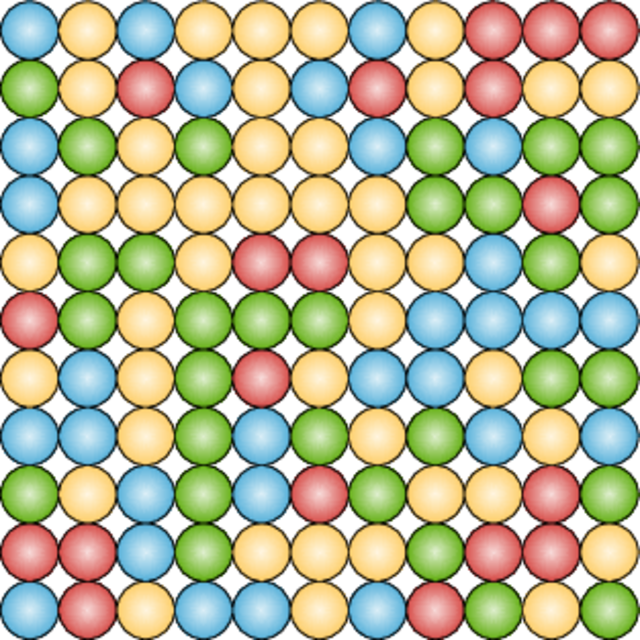
\includegraphics[width=4.5cm]{raw64.png}};
    \node[anchor=south, inner sep=0] at (1.5,5) {\bfseries{Raw data}};
  \end{scope} 

  
  \begin{scope}[
      yshift=-90,every node/.append style={
        yslant=0.5,xslant=-1},yslant=0.5,xslant=-1
    ]
    \fill[white,fill opacity=0.9] (0,0) rectangle (5,5);
    \draw[black, dashed, ultra thick] (0,0) rectangle (5,5);
    \node[anchor=south, inner sep = 0]  at (2.5,0) {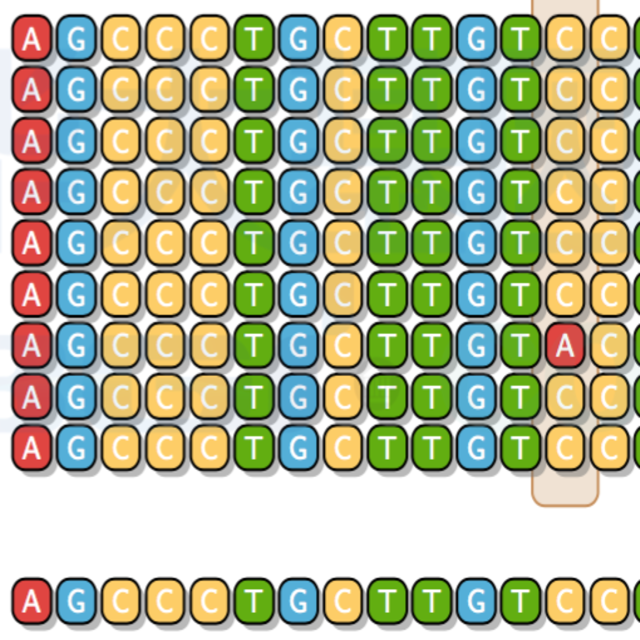
\includegraphics[width=4.5cm]{align64.png}};
    \node[anchor=south, inner sep=0] at (1.5,5) {\bfseries{Mapping}};
  \end{scope}

  \begin{scope}[
      yshift=0,every node/.append style={
        yslant=0.5,xslant=-1},yslant=0.5,xslant=-1
    ]
    \fill[white,fill opacity=.9] (0,0) rectangle (5,5);
    \draw[black, dashed, ultra thick] (0,0) rectangle (5,5);
    \node[anchor=south, inner sep = 0]  at (2.5,0) {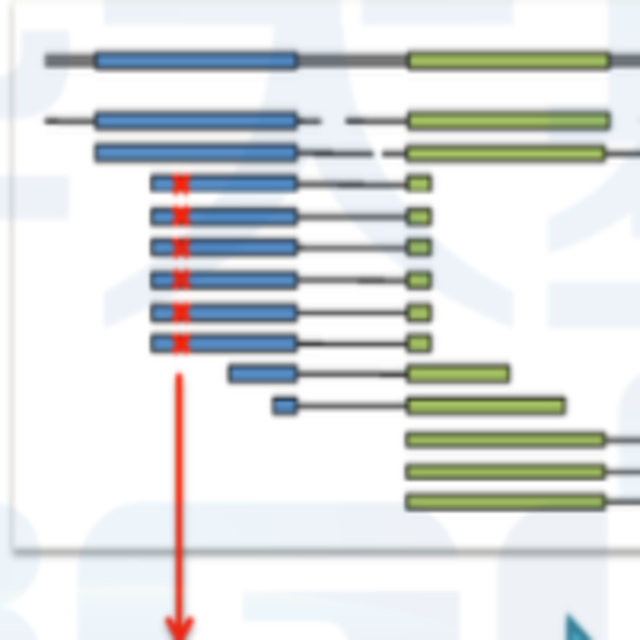
\includegraphics[width=4.5cm]{rmdup64.png}};
    \node[anchor=south, inner sep=0] at (1.5,5) {\bfseries{RM duplicates}};
  \end{scope}

  \begin{scope}[
      yshift=90,every node/.append style={
        yslant=0.5,xslant=-1},yslant=0.5,xslant=-1
    ]
    \fill[white,fill opacity=.9] (0,0) rectangle (5,5);
    \draw[black, dashed, ultra thick] (0,0) rectangle (5,5);
    \node[anchor=south, inner sep = 0]  at (2.5,0) {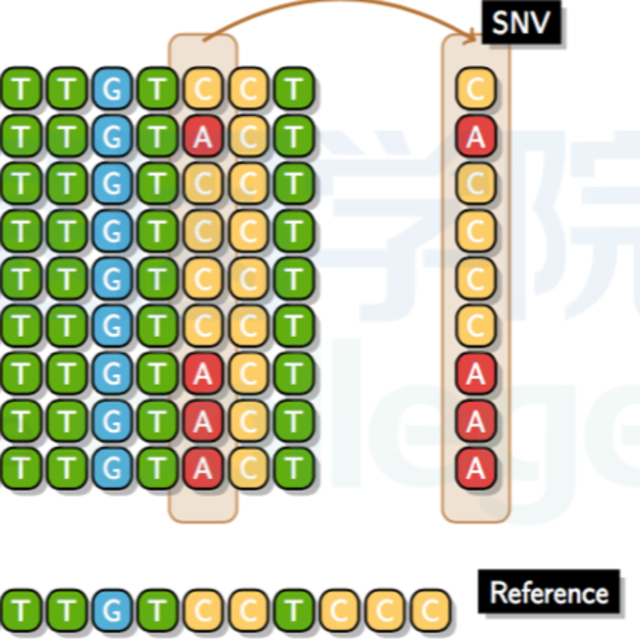
\includegraphics[width=4.5cm]{calling64.png}};
    \node[anchor=south, inner sep=0] at (1.5,5) {\bfseries{Variants Calling}};
  \end{scope}

  \begin{scope}[
      yshift=170,every node/.append style={
        yslant=0.5,xslant=-1},yslant=0.5,xslant=-1
    ]
    \fill[white,fill opacity=0.6] (0,0) rectangle (5,5);
    \draw[black, dashed, ultra thick] (0,0) rectangle (5,5);
    \node[anchor=south, inner sep = 0]  at (2.5,0) {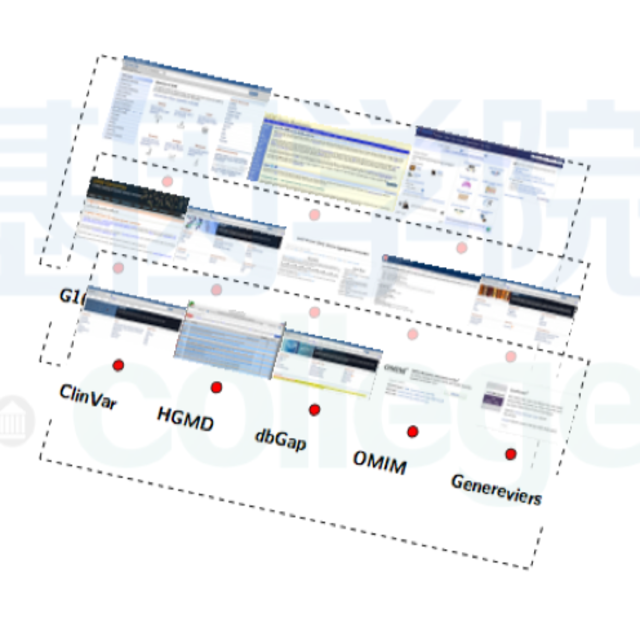
\includegraphics[width=4.5cm]{anno64.png}};
    \node[anchor=south, inner sep=0] at (1.5,5) {\bfseries{Annotation}};
  \end{scope}

 
\end{tikzpicture}

\end{document}
